\documentclass[11pt]{exam}
\usepackage[margin=1in]{geometry}
\pagestyle{plain}
\usepackage{amsmath,amsfonts,amssymb,amsthm,enumerate}
\usepackage{multicol}
\usepackage[]{graphicx}
\usepackage{hyperref}
\usepackage{tikz}
\usepackage{pgfplots}
\usepackage{subfigure}
\usepackage[final]{pdfpages}

\addtolength{\footskip}{2\baselineskip} % to lower the page numbers
\title{\vspace{-0.5in} Math 115 \\ Worksheet Section 2.6}
\date{}


% \theoremstyle{definition}
% \newtheorem{problem}{Problem}
\renewcommand{\questionlabel}{\textbf{Problem~\thequestion.}}
%\printanswers

\begin{document}
\maketitle
\vspace{-0.75in}
\section*{Warm-up questions}

\noindent
What does it mean for a function to be differentiable?

\noindent
Give an example of function that is not differentiable at a point.
\begin{solution}
  \(f(x)\) is not differentiable at \(x=0\) if \[
    \lim_{h \to 0} \frac{f(a+h)-f(a)}{h} \text{ does not exist.}
  \]
  An example of such a situation is \(f(x)=|x|\) at \(x=0\).
\end{solution}

\vspace{2.5em}
\begin{questions}
  \question The graph of $y=x^3-9x^2-16x+1$ has tangent lines with a
    slope of 5 at two points.  Find the coordinates of these points.
    \begin{solution}
      We compute
      \begin{align*}
        \frac{dy}{dx} = 3x^2-18x-16
      \end{align*}
      Next, since the derivative is the slope of the tangent line at
      \((x,y)\), we must set \(\frac{dy}{dx}=5\) and solve.
      \begin{align*}
        3x^2-18x-16=5
        & \implies 3x^2-18x-21 = 0\\
        & \implies (3x+3)(x-7) = 0\\
        & \implies x=-1 \text{ or }x=7
      \end{align*}
      Now, we find the \(y\)-coordinates
      \begin{align*}
        x = -1
        & \implies y = (-1)^3-9(-1)^2-16(-1)+1 = -3-9+16+1 = 7\\
        x = 7
        & \implies y = (7)^3-9(7)^2-16(7)+1 = 3(343) - 9(49) -
          16(7)+1 = -209
      \end{align*}
      Thus, the coordinates of the desired points are \((-1,7)\) and \((7,-209)\).
    \end{solution}
  \question The height of a sand dune (in cm) is represented by
    $f(t)=700-3t^2$, where $t$ is measured in years since 2005.
    \begin{parts}
    \part Find $f(5)$.
    \part Find $f'(5)$.
    \part Provide practical interpretations of these two quantities.
    \end{parts}
    \begin{solution}
      \begin{enumerate}[(a)]
      \item \(f(5) = 700-3(5)^2 = 625\)
      \item \(f'(t) = -6t \implies f'(5) = -6(5) = -39\)
      \item \(f(5)\): In 2010, the height of the sand dune is 625cm.\\
        \(f'(5)\): From January 2010 to February 2010, the sand dune's
        height will decrease by about \(3.25\)cm.
      \end{enumerate}
    \end{solution}
  \question Using a graph to help you, find the equations of all lines through the origin tangent to the parabola $$y=x^2-2x+4.$$  Sketch the lines on your graph.
    \begin{solution}
     We need points \((a,f(a))\) such that the line from \((0,0)\) to
     \((a,f(a))\) have slope \(f'(a)\). Thus, we must solve
     \(\frac{f(a)}{a} = f'(a)\). We check
     \begin{align*}
       f'(x) = 2x-2\\
       \frac{f(a)}{a} = f'(a)
       & \implies \frac{a^2-2a+4}{a} = 2a-2 
       & \implies a^2-2a+4 = 2a^2-2a\\
       & \implies -a^2+4 = 0 \\
       & \implies a^2 = 4 \\
       & \implies a = \pm 2
     \end{align*}
     Thus, there will be two such lines. Since they both pass through
     the origin, we know their \(y\)-intercept is \(0\) and we need
     only solve for their slopes.
     \begin{align*}
       a = -2 \implies f'(-2) = 2(-2)-2 = -6 \implies y = -6x\\
       a = 2 \implies f'(2) = 2(2) -2 = 2 \implies y = 2x
     \end{align*}
     Thus, the equations of the two lines are \(y=2x\) and \(y=-6x\).
     \begin{center}
      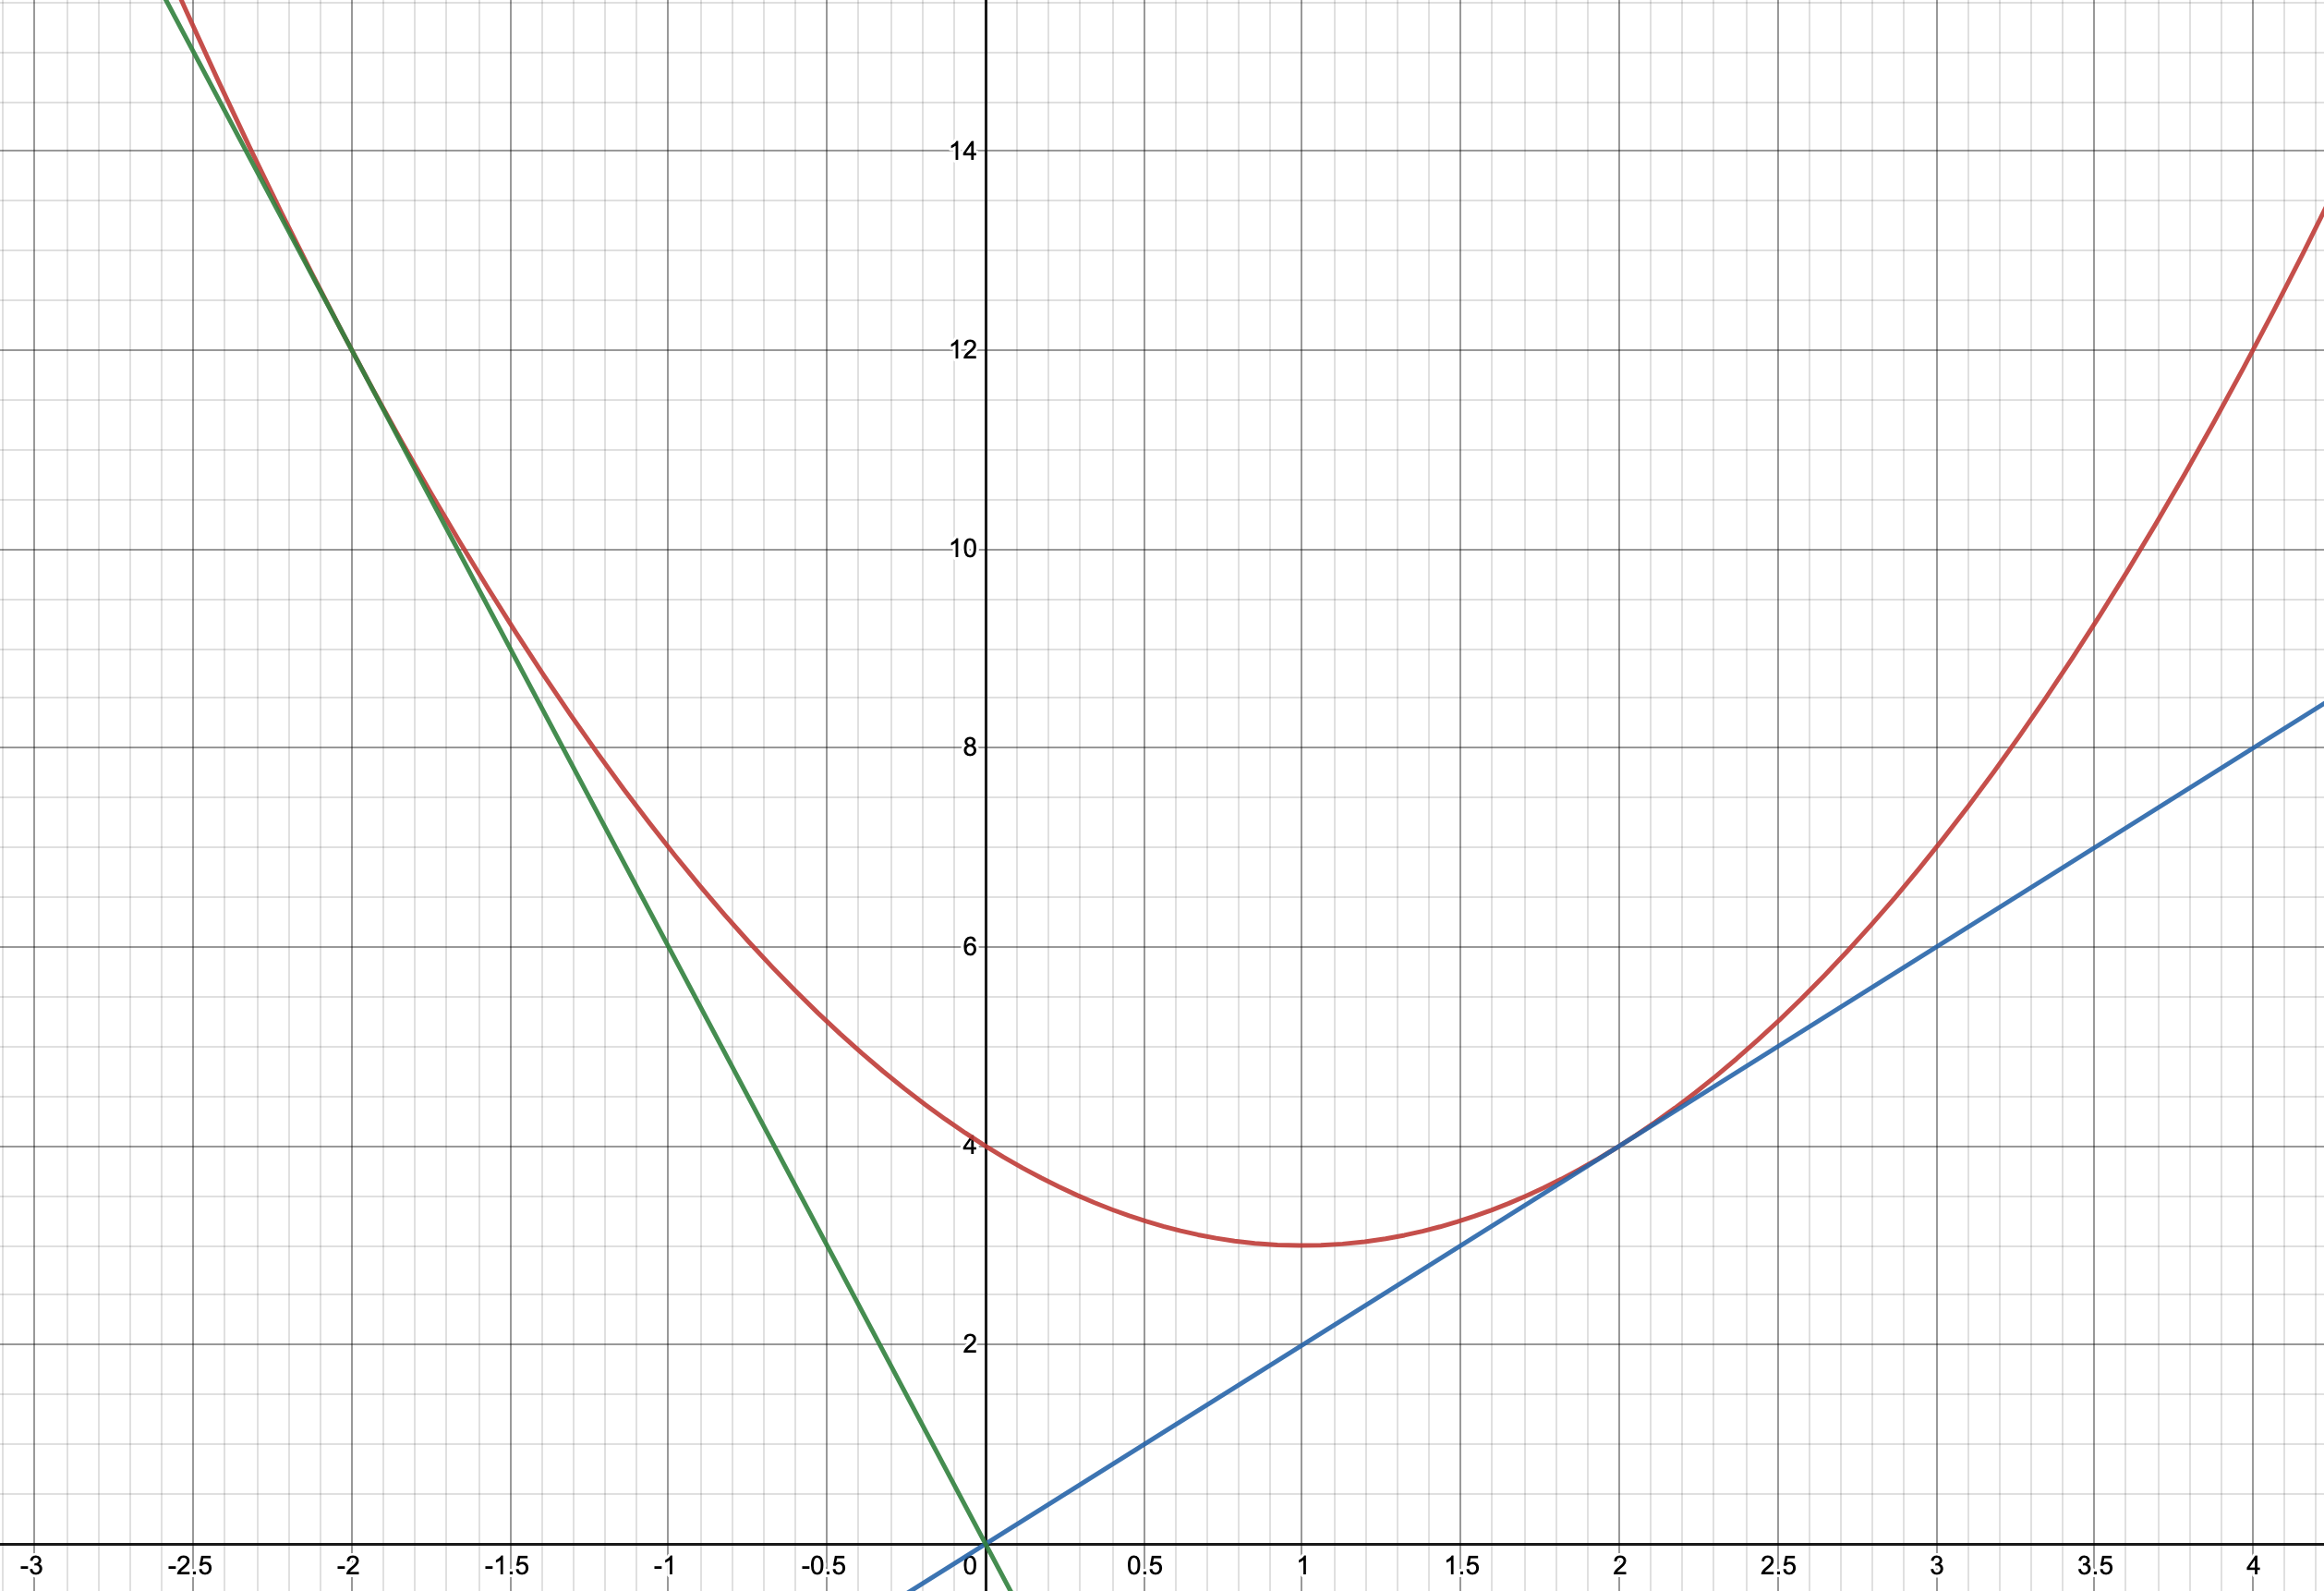
\includegraphics[scale=0.3]{parabola_with_tangents}
     \end{center}
    \end{solution}
  \question (Fall 2016 Exam 2) The graph of a function $f$ is shown below.
    \begin{center}
      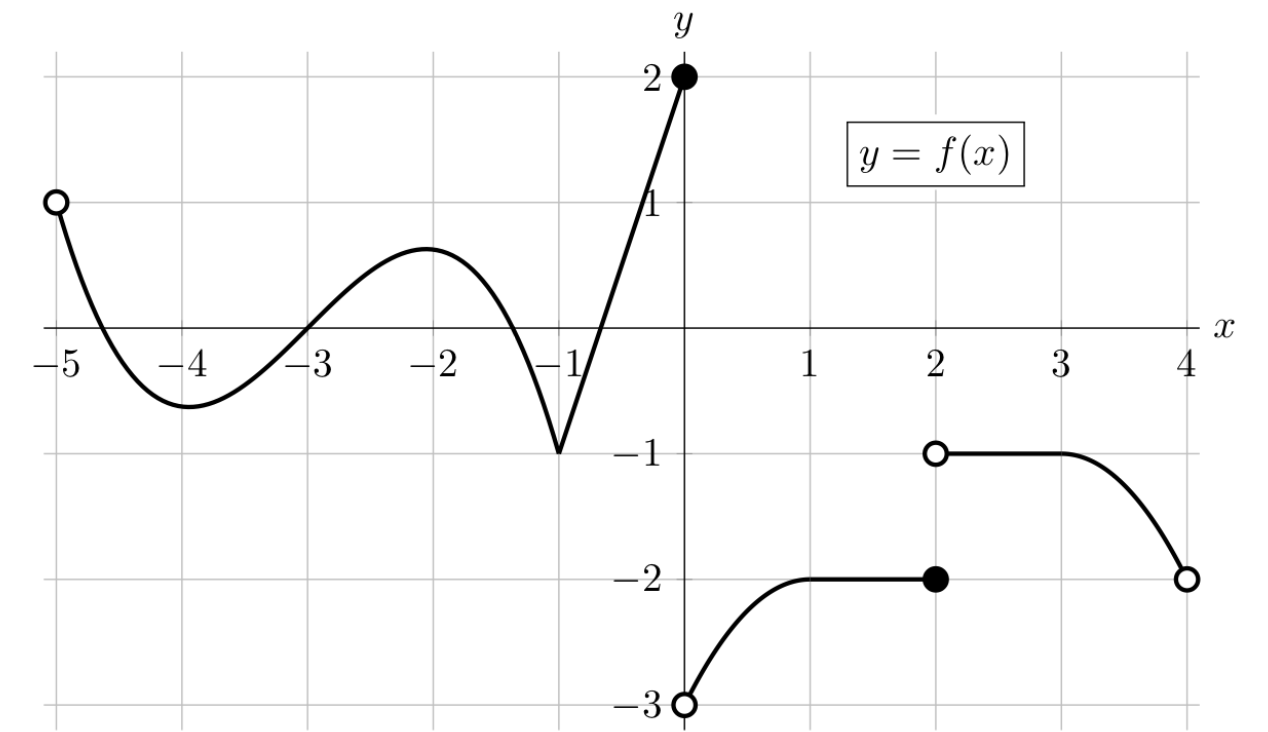
\includegraphics[scale=0.6]{graphf.png}
    \end{center}
    Sketch a graph of $f'(x)$ (the derivative of the function $f(x)$) on the interval
$-5 < x < 4$. Be sure that you pay close attention to each of the following:
 \begin{itemize}
\item Where $f'$ is defined.
\item The value of $f'(x)$ near each of $x = -5, -4, -3, -2, -1, 0, 1, 2, 3, 4$.
\item The sign of $f'$.
\item Where $f'$ is increasing/decreasing/constant.
\end{itemize}
\begin{solution}
 See \href{https://dhsp.math.lsa.umich.edu/exams/115exam2/f16/s4.pdf}{https://dhsp.math.lsa.umich.edu/exams/115exam2/f16/s4.pdf}  
\end{solution}
\vspace{1.5in}
\question (Winter 2014 Exam 2) The graph of a function $g$ is shown below.
  \begin{center}
  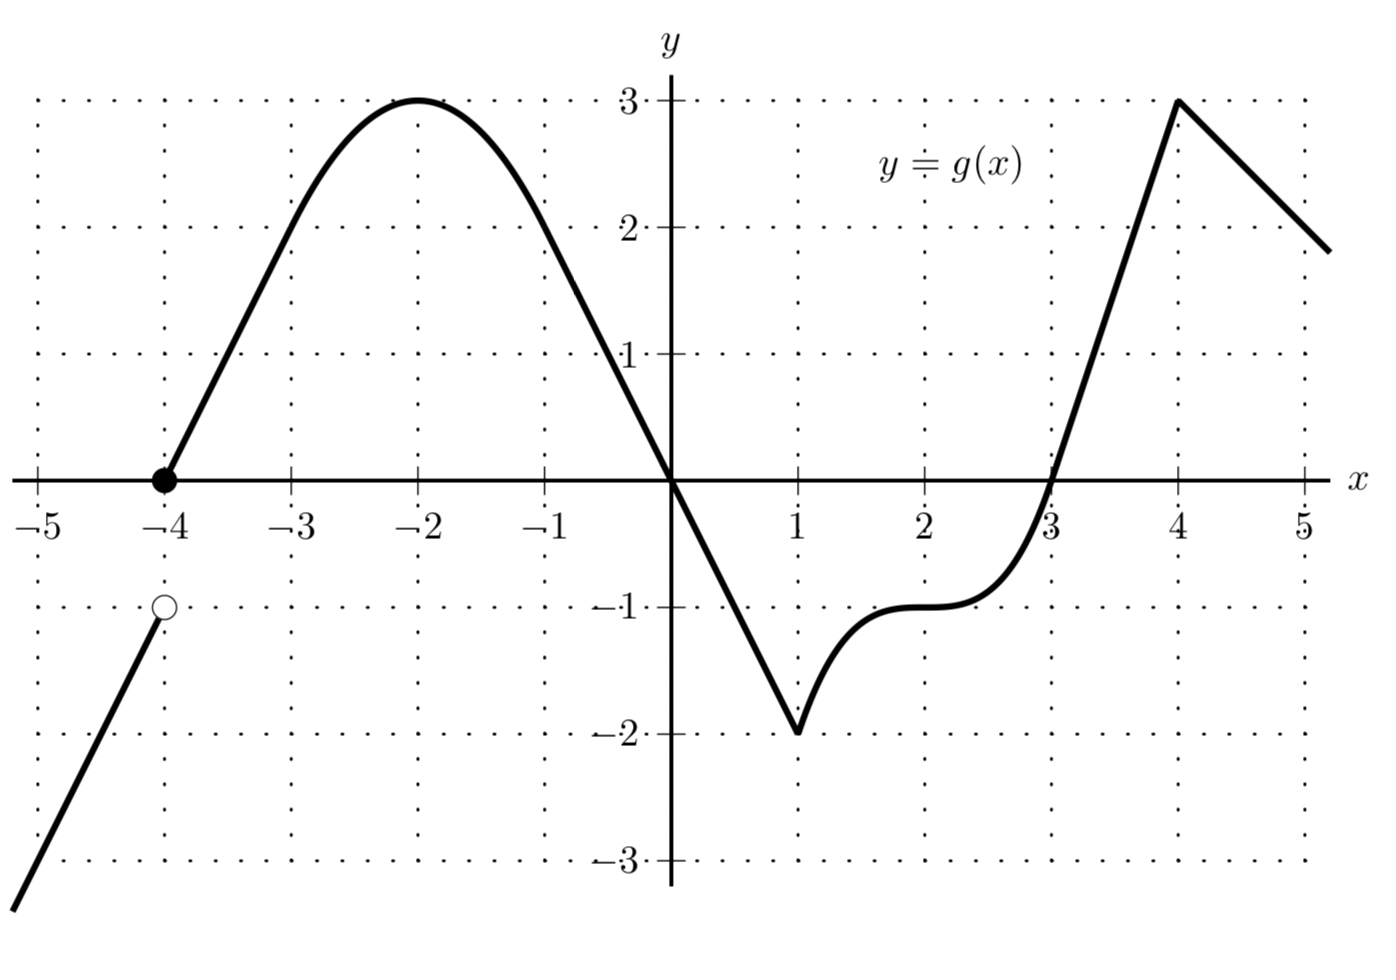
\includegraphics[scale=0.4]{graphg.png}
  \end{center}
Sketch the graph of y = $g'(x)$. Be sure that you pay close attention to each of the following:
\begin{itemize}
\item Where $g'$ is defined.
\item the value of $g'(x)$ near each of $x = -5,-4,-3,-2,-1,0,1,2,3,4,5$
\item The sign of $g'$.
\item Where $g'$ is increasing/decreasing/constant.
\end{itemize}
\begin{solution}
  See \href{https://dhsp.math.lsa.umich.edu/exams/115exam2/w14/s6.pdf}{https://dhsp.math.lsa.umich.edu/exams/115exam2/w14/s6.pdf}
\end{solution}
\end{questions}
\end{document}
%%% Local Variables:
%%% mode: latex
%%% TeX-master: t
%%% End:
